% -*- LaTeX -*-
% -*- coding: utf-8 -*-
%
% michael a.g. aïvázis
% california institute of technology
% (c) 1998-2012 all rights reserved
%

\lecture{Introduction to \pyre}{20120518}

% --------------------------------------
% namespace design
\begin{frame}[fragile]
%
  \frametitle{Namespace design}
%
  we are now in a position to assemble the package \package{gauss}; let's start by laying out
  the package namespace
%
  \begin{figure}
    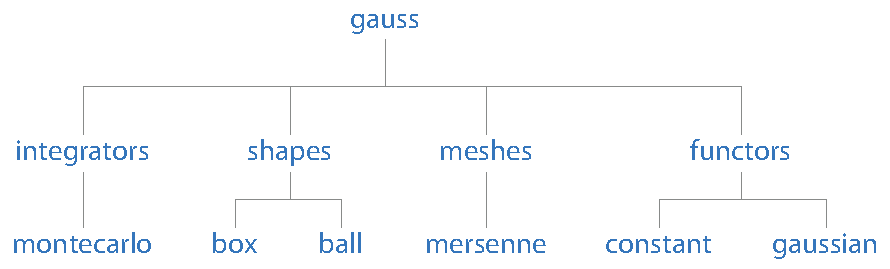
\includegraphics[scale=0.5]{figures/gauss-namespace.pdf}
  \end{figure}
%
  and try to use this layout for both the logical and physical structure
  \begin{itemize}
  \item the top level is our package name
  \item the internal nodes become the names of interfaces and subdirectories
  \item the leaves are the component family names and the names by which the component
    factories are accessible
  \end{itemize}
%
\end{frame}

% --------------------------------------
% shape as a package
\begin{frame}[fragile]
%
  \frametitle{The \package{shapes} package}
%
  in order to make the directory \srcfile{gauss/shapes} a python package, we need to create
  the special file \srcfile{gauss/shapes/\_\_init\_\_.py}
%
  \python{firstnumber=9,linerange={9-18}}{listings/gauss/shapes/__init__.py}
%
  the \keyword{import} statements 
  \begin{itemize}
  \item use \emph{local} imports to make sure that we are accessing the correct modules
  \item create local names for the classes declared inside the named modules
  \end{itemize}
%
  the net effect is to simplify access to the components 
%
  \begin{ipython}{}
    from gauss.shapes import box, ball
  \end{ipython}
\end{frame}

% --------------------------------------
% shapes
\begin{frame}[fragile]
%
  \frametitle{Shapes}
%
  the \interface{Shape} interface in \srcfile{gauss/shapes/Shape.py}
%
  \python{firstnumber=9,linerange={9-37},basicstyle=\tt\tiny}{listings/gauss/shapes/Shape.py}
%
\end{frame}

% --------------------------------------
% from disks to d-spheres
\begin{frame}[fragile]
%
  \frametitle{From disks to spheres in $d$ dimensions}
%
  \begin{itemize}
%
  \item for the simple shapes, such as boxes and disks, it is easy to generalize to arbitrary
    dimensions
    \begin{itemize}
    \item for our purposes, this is useful mostly as an exercise in operating on containers
    \end{itemize}
%
  \item the volume of a sphere of radius $r$ in $d$ dimensions is given by
%
    \[
    \mu_{d}(r) = \frac{\pi^{\frac{d}{2}}}{\Gamma\left(\frac{d}{2} + 1\right)} r^{d}
    \]
%
    for even $d$
    \[
    \mu_{d}(r) = \frac{\pi^{\frac{d}{2}}}{\left(\frac{d}{2}\right)!} r^{d}
    \]
%
    for odd $d$
    \[
    \mu_{d}(r) = \frac{2^{\frac{d+1}{2}} \pi^{\frac{d-1}{2}}}{d!!} r^{d}
    \]
%
  \end{itemize}
%
\end{frame}

% --------------------------------------
% balls
\begin{frame}[fragile]
%
  \frametitle{Ball}
%
  the implementation of \component{Ball} in \srcfile{gauss/shapes/Ball.py}
%
  \python{firstnumber=9,linerange={9-42},basicstyle=\tt\tiny}{listings/gauss/shapes/Ball.py}
%
\end{frame}

% --------------------------------------
% balls
\begin{frame}[fragile]
%
  \frametitle{Ball - continued}
%
  \python{firstnumber=43,linerange={43-60}}{listings/gauss/shapes/Ball.py}
%
\end{frame}

% --------------------------------------
% boxes
\begin{frame}[fragile]
%
  \frametitle{Box}
%
  the implementation of \component{Box} in \srcfile{gauss/shapes/Box.py}
%
  \python{firstnumber=9,linerange={9-30}}{listings/gauss/shapes/Box.py}
%
\end{frame}

% --------------------------------------
% boxes
\begin{frame}[fragile]
%
  \frametitle{Box - continued}
%
  \python{firstnumber=33,linerange={33-60}}{listings/gauss/shapes/Box.py}
%
\end{frame}

% --------------------------------------
% meshes
\begin{frame}[fragile]
%
  \frametitle{The \package{meshes} package}
%
  again, we need the special file \srcfile{gauss/meshes/\_\_init\_\_.py} in order to turn
  \srcfile{gauss/meshes} into a python package
%
  \python{firstnumber=9,linerange={9-17}}{listings/gauss/meshes/__init__.py}
%
\end{frame}

% --------------------------------------
% point clouds
\begin{frame}[fragile]
%
  \frametitle{Point clouds}
%
  the \interface{PointCloud} interface in \srcfile{gauss/meshes/PointCloud.py}
%
  \python{firstnumber=9,linerange={9-33}}{listings/gauss/meshes/PointCloud.py}
%
\end{frame}

% --------------------------------------
% the built-in random number generator
\begin{frame}[fragile]
%
  \frametitle{Generating points with the Mersenne Twister RNG}
%
  in \srcfile{gauss/meshes/Mersenne.py}
%
  \python{firstnumber=9,linerange={9-34}}{listings/gauss/meshes/Mersenne.py}
%
\end{frame}

% --------------------------------------
% functors
\begin{frame}[fragile]
%
  \frametitle{The \package{functors} package}
%
  the package initialization file in \srcfile{gauss/functors/\_\_init\_\_.py} 
%
  \python{firstnumber=9,linerange={9-18}}{listings/gauss/functors/__init__.py}
%
\end{frame}

% --------------------------------------
% functors
\begin{frame}[fragile]
%
  \frametitle{Functors}
%
  the \interface{Functor} interface in \srcfile{gauss/functors/Functor.py}
%
  \python{firstnumber=9,linerange={9-30}}{listings/gauss/functors/Functor.py}
%
\end{frame}

% --------------------------------------
% the constant functor
\begin{frame}[fragile]
%
  \frametitle{The \component{Constant} functor}
%
  in \srcfile{gauss/functors/Constant.py}
%
  \python{firstnumber=9,linerange={9-33}}{listings/gauss/functors/Constant.py}
%
\end{frame}

% --------------------------------------
% gaussians
\begin{frame}[fragile]
%
  \frametitle{A non-trivial functor}
%
  \python{firstnumber=9,linerange={9-26}}{listings/gauss/functors/Gaussian.py}
%
\end{frame}

% --------------------------------------
% gaussians
\begin{frame}[fragile]
%
  \frametitle{A non-trivial functor -- continued}
%
  \python{firstnumber=29,linerange={29-51}}{listings/gauss/functors/Gaussian.py}
%
\end{frame}

% --------------------------------------
% integrators
\begin{frame}[fragile]
%
  \frametitle{The \package{integrators} package}
%
  the package initialization file in \srcfile{gauss/integrators/\_\_init\_\_.py} 
%
  \python{firstnumber=9,linerange={9-17}}{listings/gauss/integrators/__init__.py}
%
\end{frame}

% --------------------------------------
% integrators
\begin{frame}[fragile]
%
  \frametitle{Integrators}
%
  in \srcfile{gauss/integrators/Integrator.py}
%
  \python{firstnumber=9,linerange={9-39},basicstyle=\tt\tiny}{listings/gauss/integrators/Integrator.py}
%
\end{frame}

% --------------------------------------
% monte carlo
\begin{frame}[fragile]
%
  \frametitle{The Monte Carlo integrator}
%
  in \srcfile{gauss/integrators/MonteCarlo.py}
%
  \python{firstnumber=9,linerange={9-36},basicstyle=\tt\tiny}{listings/gauss/integrators/MonteCarlo.py}
%
\end{frame}

% --------------------------------------
% monte carlo -- continued
\begin{frame}[fragile]
%
  \frametitle{The Monte Carlo integrator -- continued}
%
  \python{firstnumber=38,linerange={38-53}}{listings/gauss/integrators/MonteCarlo.py}
%
\end{frame}

% --------------------------------------
% gauss
\begin{frame}[fragile]
%
  \frametitle{Top level -- the \package{gauss} package}
%
  the package initialization file in \srcfile{gauss/\_\_init\_\_.py} 
%
  \python{firstnumber=9,linerange={9-38},basicstyle=\tt\tiny}{listings/gauss/__init__.py}
%
\end{frame}

% end of file 
